\chapter{Introduzione}
Questo capitolo introduce le componenti principali del progetto ed ha il compito di spiegare in maniera approfondita le operazioni svolte da esse.
Tali componenti sono state raggruppate nei tre campi su cui è stato condotto il lavoro: bioinformatica, sviluppo informatico e i dispositivi low power.

Il primo di questi è il campo bioinformatico e, quindi, un approfondimento del metodo GATK-LOD\ped{n} riguardante la ricerca sull'origine dei tumori attraverso procedure di natura bioinformatica.
Inoltre, sarà sottolineata l'importanza della fisica nell'ambiente di lavoro e nella creazione degli algoritmi.

Il secondo è il campo di sviluppo informatico, ovvero la spiegazione del programma Snakemake, le cui funzionalità concendono ampie possibilità sulla gestione delle risorse offerte dalle macchine.

Il terzo è il campo dei dispositivi low power, accompagnati dalla descrizione di coloro che sono stati adoperati per la computazione.

La combinazione tra tali differenti ambiti ha quindi fornito i sufficienti elementi per proseguire con la costruzione e la seguente attuazione del programma; i quali saranno affrontati nel prossimo capitolo.


\section{La ricerca delle mutazioni genetiche}
Questa sezione si occuperà di dare un'idea generale su un ramo degli studi riguardanti le mutazioni genetiche che sviluppano e alimentano i tumori.

Negli ultimi anni l'indagine sulle forme cancerogene basata sulle variazioni che avvengono nel codice genetico ha suscitato sempre più interesse e ciò ha portato allo sviluppo di un discreto numero di programmmi, algoritmi e metodi atti all'analisi del DNA.
Ognuna di queste applicazioni ha come fine la determinazione di quelle mutazioni nei geni che comportano l'insorgere delle malattie tumorali ora conosciute.
La conoscenza di una tale correlazione è di vitale importanza per la pianificazione di un piano di cura adeguato e, in altri casi, per un intervento anticipato in grado di prevenire il presentarsi della malattia.

Un altro aspetto delicato è la risposta del cancro alle cure a cui è sottoposto il paziente e che, in taluni casi, si concretizza in una forma di resistenza a questi interventi, come ad esempio la resistenza alla chemioterapia.
La gestione di una tale conseguenza può essere aiutata dalla piena comprensione dell'origine genetica del tumore, la quale agevolerebbe la scelta tra i percorsi di guarigione più opportuni.

Seppur avendo lo stesso obiettivo, gli innumerevoli algoritmi utilizzati spesso si ritrovano in contrasto tra di loro e queste discrepanze sono rilevate quando si procede con il confronto dei risultati finali, che solitamente o non concordano o sono proprio differenti.
Questi algoritmi elaborano i dati sperimentali grezzi attraverso vari processi che, generalmente, sfruttano svariati metodi di statistica le cui radici provengono dai campi di matematica e fisica applicata.
La netta differenza di prestazioni, insieme alle diverse metodologie operate, lascia ai gruppi di ricerca un arduo compito nella scelta del metodo più idoneo da applicare.

In questa tesi il metodo considerato prende il nome di GATK-LOD\ped{n} ed è ideato dalla combinazione di due tra i tools più comuni nel panorama bioinformatico: GATK e MuTect.
Prima di esporre questo algoritmo e le sue fondamenta, è necessario definire il percorso storico che ha determinato le moderne tecniche con cui è analizzato attualmente il materiale genetico e le caratteristiche generali di questi procedimenti.
Inoltre, sarà sottolineato l'impatto della fisica nei campi della biologia e della medicina.

\subsection{L'analisi del DNA}
Lo studio sull'eredità genetica ha inizio con gli studi di Gregory Mendel nella seconda metà del diciannovesimo secolo e, nella prima metà del secolo seguente, un serie di contributi, tra cui la fotografia della doppia elica da parte di Roselind Franklin, pongono le basi alla moderna ricerca genetica.
Il contributo essenziale è la determinazione della struttura del DNA a cui contribuirono James Watson e Francis Crick, la quale permise di cominciare la decifrazione del codice genetico.
I tentativi di decodifica hanno subito una svolta significativa nel 
977 grazie alla tecnica di sequenziamento genetico proposta dal biochimico Frederick Sanger, conosciuta ora come metodo Sanger.
Tale procedimento determina l'ordine delle basi in un filamento breve di DNA utilizzando la tecnica dell'elettroforesi e il supporto di alcuni marcatori radioattivi.
Questo metodo è considerato rivoluzionario ed è stato utilizzato come capostipite del sequenziamento del genoma umano per più di 40 anni.

Nel 1984 il Department of Energy (DOE) e il National Institutes of Health (NIH) degli Stati Uniti hanno avviato un programma per lo sviluppo di tecnologie e metodi per il sequenziamento genetico e la mappatura del codice genetico umano: lo Human Genome Project(HGP).
L'obiettivo essenziale del programma è la decodifica del DNA umano che comprende principalemente la determinazioni delle sequenze, cioè l'ordine delle basi, e la mappatura dei geni, ovvero la localizzazione dei geni per la maggior parte dei cromosomi e le connessioni con le caratteristiche fisiche e germinali.
Oltre a ciò, il progetto ha cercato di analizzare anche i genomi di esseri viventi valutati più semplici, come ad esempio le mosche.

Molte tecniche per la trattazione del materiale genetico hanno partecipato alla ricerca, ma il primo procedimento attuato dall'HGP fu il BAC, Bacterial Artificial Chromosome, che sfruttava la clonazione apportata da certi batteri per ottenere un numero elevato di filamenti.
Quest'ultimi subivano un ulteriore frammentazione, per poi essere sequenziati con il metodo Sanger ed infine essere riuniti per formare l'unica stringa di DNA.

Dopo oltre un decennio, nell'Aprile del 2003, l'HGP si è concluso con successo, essendo stato decodificato il 99\verb!%! del genoma umano e visto che gli studi erano stati allargati prematuramente ad altri interessi, soprattutto nelle ricerche sulle malattie.
Da quel momento in poi, il termine comune affiliato alle nuove tecniche sul genoma umano è Next-Generation Sequencing(NGS), di cui fanno parte gli algoritmi coinvolti in questa presentazione.

\subsubsection{NGS}
La necessità di garantire una maggior rapidità, e anche di ridurre le spese, ha aperto un altro capitolo nella ricerca sul genoma umano: il Next-Generation Sequecing\cite{Behjati2013}.
Tale necessità deriva dal fatto che il metodo Sanger, per via di un esaminazione estremamente precisa, ha ottenuto l'intero genoma umano in circa tredici anni sostenuto da un investimento che si aggira attorno ai $\$\,2.7$ miliardi. 
Questa nuova generazione di tecnologie, che sfrutta la parallelizzazione di processi su scale microscopiche \cite{Shendure2008}, concede ai ricercatori strumenti estremamente più veloci, tali da stimare il genoma di un individuo in meno di un giorno, e molto meno costosi.
In aggiunta, i numerosi metodi sviluppati all'interno del NGS sono fortemente radicati sulla teoria dei network, la quale è una branca della fisica che ha subito nell'ultimo ventennio un notevole progresso e che ha acquistato un significato oramai fondamentale nella ricerca medica e biologica. 

Un fattore importante che supporta lo sviluppo di tecnologie più veloci è l'esistenza del genoma di riferimento prodotto dal HGP, che permette il confronto di sole certe regioni senza quindi dover estrarre l'intero codice genetico.
Un ulteriore contributo è dato anche dalla contemporanea crescita delle aree che cooperano con la biologia, come ad esempio le tecniche di computazione.

Questi strumenti sono più conveniente del metodo Sanger, il quale rimane comunque artefice di un eccellente connubio tra qualità e quantità di letture(read-lenght), ma devono trovare l'idoneo compromesso tra l'accuratezza dei risultati e la diminuzione delle spese temporali ed economiche.
Infatti, nello studio di sequenze a piccola scala la tecnologia di Sanger resta tuttora una tra le più affidabili, mentre su letture ad ordini superiori è atteso che le applicazioni del NGS possano vantare in futuro la miglior proficuità.

Pur adoperando tipi di tecnologia diversi, il funzionamento di un generale algoritmo del NGS prevede sempre alcuni passaggi, tra cui l'allineamento delle letture con un riferimento e l'investigazione sulle possibili variazioni.
La difficoltà nello scegliere quale tra le diverse opzioni disponibili usare può è superata dal confronto tra i diversi risultati finali dei procedimenti, ovviamente in relazione agli scopi preposti. 
Essi includono la qualità dei risultati, le tempistiche previste e altre caratteristiche come l'assemblaggio e gli allineamenti.

Negli ultimi anni si sono aggiunti alle ricerche del NGS due software chiamati GATK e MuTect, i cui metodi hanno condotto allo sviluppo dell'algoritmo coinvolto nella ricerca presentatata in questa tesi: il GATK-LOD\ped{n}.


\subsection{Il metodo GATK-LOD\ped{n} e le sue radici}
L'ideazione di questo algoritmo é dovuta ad un gruppo di ricercatori del Dipartimento di Fisica e Astronomia dell'Università di Bologna nell'ambito dello studio sulla scoperta di polimorfismi somatici del singolo nucleotide nel sequenziamento dell'esoma \cite{DoValle2016}.
Precisamente, questo genere di polimorfismo è denonimato con la sigla SNP, single nucleotide polymorphism, e indica quelle variazioni nei singoli nucleotidi che si verificano con frequenza significativa in una specifica posizione del genoma.
In particolare, l'esoma comprende quelle regioni del genoma in cui sono codificate le istruzioni per l'RNA e per la sintesi delle proteine.

Le mutazioni genetiche si distinguono in due tipologie: germinali e somatiche. Le prime identificano le variazioni nei cromosomi determinanti il sesso dell'individuo e che si trasmettono di generazione in generazione. Le seconde, invece, rappresentano le variazioni negli altri cromosomi contenenti le caratteristiche del singolo soggetto. 
L'algoritmo GATK-LOD\ped{n} si focalizza sulle mutazioni somatiche perchè esse hanno un ruolo chiave nella progressione della malattia e nella resistenza alla chemioterapia.

L'interesse nel proporre questo metodo nasce dal desiderio di poter predisporre di uno strumento che non si aggiunga al gruppo di software già esistenti, bensì che ottimizzi e potenzi alcuni tra questi.
E' per questo che il team di studiosi ha considerato due applicazioni standard, GATK e MuTect, e li ha composti in modo da migliorare i prodotti finali di entrambi.
Infatti alla completa esecuzione di GATK è stato applicato una componente di MuTect, ovvero un classificatore Bayesiano conosciuto come LOD\ped{n}, il cui scopo è verificare un ulteriore volta i risultati ottenuti.
I passaggi previsti dall'algoritmo sono vari e di seguito saranno esposti coloro ritenuti più rilevanti.

Dopo aver raccolto i campioni normali e quelli per alcune specie di tumori attraverso specifiche metodologie sperimentali, essi sono stati sottoposti ad un controllo di qualità tale da rimuovere le letture considerate a bassa confidenza.
A questo punto, sono state applicati in successione i tools BWA-MEM e Picard, dove il primo allinea le reads e il secondo le ordina, indicizza e in più ne marca i duplicati.
Una volta completata una nuova fase di riallineamento locale e di ricalibrazione sulla qualità delle letture, grazie all'utilizzo di alcuni strumenti del Genome Analysis Toolkit, sono stati eseguiti GATK e MuTect per la ricerca delle varianti sui singoli nucleotidi(SNV).

La differenza procedurale tra queste due applicazioni è che, mentre MuTect ritrova le mutazioni contemporaneamente tra i campioni normali e tumorali, GATK le chiama indipendentemente.
Un'osservazione da sottolineare è che i due metodi scovano pure varianti che non sono condivise da entrambi, indicando la natura incompleta dei sistemi utilizzati.
Un ulteriore distinzione tra GATK e MuTect è data dal tipo di risultati raccolti poichè, se il primo è dotato di una maggiore sensibilità alle mutazioni, dalle 3 alle 20 volte superiore al secondo, quest'ultimo possiede una maggiore specificità degli SNVs.
Avendo GATK un elevato numero di falsi positivi nella chiamata alle varianti, è stato aggiunto in fondo all'algoritmo il classificatore Bayesiano di MuTect per cercare di ridurre questo errore.
Il compito del LOD\ped{n} consiste nel calcolare il rapporto tra i due seguenti eventi probabilistici.
Il primo è il caso in cui le mutazioni nel campione normale siano dovute a rumori di fondo e quindi in realtà non esistano.
Il secondo, invece, considera il caso in cui la mutazione esista davvero nel campione normale e sia dovuta ad una variante germinale eterozigote.
A questo punto, se il rapporto tra le probabilità (il Log Odds, da cui la sigla LOD) eccede un valore di soglia fissato, il classificatore definisce la variante come somatica.

Nella ricerca sono stati confrontati i prodotti finali dei tre algoritmi ed è stato verificato che l'uso di GATK-LOD\ped{n} riduce notevolmente il numero di chiamate degli SNVs di GATK, mantenendo una sensibilità nettamente superiore a MuTect.
Questa riduzione è dovuta ovviamente all'eliminazione di un sostanziale numero di falsi positivi, la cui entità dipende dalla tipologia di tumore esaminato.

Il miglioramento dei precedenti metodi, però, non si limita solo alla filtrazione dei falsi positivi ma anche al mantenimento della sensibilità di GATK e ad un aumento della specificità.
Quest'ultimo è indicato dal fatto che GATK-LOD\ped{n} abbia presentato frequenze di validità superiori e un miglior PPV(Positive Predictive Value) rispetto a GATK su vari range di VAF(Variant Allelic Frequency).
Le metodologie adoperate per confrontare la sensibilità e la specificità non sono state ritenuti utili allo scopo della presentazione e per questo non verranno trattate.

A posteriori delle indagini sperimentali, GATK-LOD\ped{n} si è rivelato uno strumento utile ad allargare le capacità di GATK e a scovare varianti non trovate da MuTect senza dover rinunciare alla specificità e sensibilità.

Visti i risultati positivi ricavati dall'algoritmo, la ricerca sostiene con un fiducia che un metodo di questo tipo possa aiutare a definire con maggior dettaglio le mutazioni somatiche di genomi cancerogeni, favorendo le valutazioni mediche e gli approcci sui percorsi di cura.

In modo da fornire una conoscenza più approndita delle operazioni che avvengono nel sequenziamento, saranno esposti %brevemente il meccanismo statistico e 
i passaggi fondamentali alla base delle applicazioni utilizzate nel metodo GATK-LOD\ped{n}: GATK e MuTect.
\begin{figure}[H]
\centering
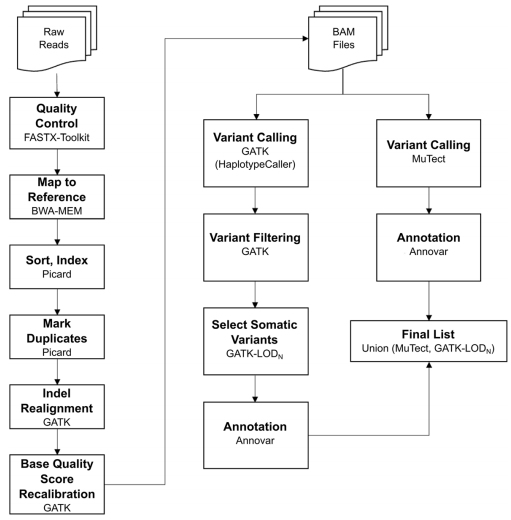
\includegraphics[scale=0.4]{GATK-LODn.png}
\caption{GATK-LOD\ped{n} Workflow}
\label{fig: GATK-LODn}
\end{figure}

%\subsection{La statistica di base}

\subsubsection{GATK}
Il Genome Analysis Toolkit è un framework di programmazione creato da un gruppo di ricercatori di Boston, Massacchussets, assieme al Broad Institute di Harvard e l'MIT in Cambridge, Massacchussets, per facilitare lo sviluppo di programmi che analizzano l'enorme mole generati dal NGS, Next Generation DNA Sequencing \cite{McKenna2010}.
Infatti, l'utilizzo di questo sistema permette di sviluppare tools più solidi e performanti per il sequenziamento genetico.

La mancanza di strumenti flessibili e sofisticati dediti alla manipolazione dei dati di sequenziamento in maniera programmatica ha portato alla creazione di GATK.
Infatti, la maggior parte dei software che supportano l'analisi del DNA concedono alte prestazioni sono nella specifica area di interesse, senza mantenerle su differenti ambiti.
Questo deficit e l'emergere di un formato specifico per i prodotti del sequenziamento (SAM), hanno dato l'opportunità di ideare un software per la semplificazione delle analisi sui set di dati.

L'architettura di base per GATK è il MapReduce, il cui funzionamento implica la separazione delle computazioni in due passaggi.
Nel primo, l'intero problema è suddiviso in tanti elementi discreti indipendenti, i quali sono correlati alla funzione Map; nel secondo step, l'operatore Reduce riunisce gli esiti di Map in un unico risultato finale.
Siccome solo in certi casi, come la ricerca degli SNPs, vi è un adattamento naturale del sistema, GATK è costruito su traversals e walkers.
Le traversals sono schemi che provvedono alla preparazione e divisione dei dati; mentre le walkers consistono nei differenti moduli di analisi che computano i dati provenienti dalle prime.
Anche se GATK ha un numero ridotto di traversals, questo basta per soddisfare le esigenze della maggior parte della comunità di ricerca.
I due trasversal standard sono il "by each sequencer read" e il "by every read covering single base position in a genome", il cui uso è sfruttato per operazioni standard come la chiamata agli SNPs.
Il meccanismo di questi schemi non è riportato poichè non è stato ritenuto necessario per la comprensione di questo scritto.

Uno dei punti di forza dell'algoritmo è la capacità di gestire l'enorme quantità di materiale ricavato dal sequenziamento.
In particolare, GATK divide il tutto in pezzi chiamati "shard" che, al contrario della maggior parte dei sistemi di suddivisione, sono di una dimensione del multikilobase.
In questo modo non sono limitate le capacità della memoria e le prestazioni nel caso di parallelismo.
Questi shards contengono tutte le informazioni della regione genomica associata e sono trasmesse al trasversal prescelto.

Altre caratteristiche di GATK sono la possibilità di selezionare solo certe regioni del genoma, la parallelizzazione delle azioni da svolgere, l'organizzazione dei files di input grazie ad un'operazione di merging e la presenza di un walker relativo alla depth of coverage(DoC).

Il metodo stima il genotipo più probabile attraverso un semplice algoritmo Bayesiano, che ha funzione sia di punto di partenza per sviluppare nuovi classificatori; che di mettere in luce le capacità di parallelizzazione e di ottimizzazione della memoria disposte da GATK.
E' importante sottolineare che è proprio la semplicità dell'operatore la causa di molti falsi positivi chiamati.

Il Genome Analysis Toolkit è quindi un framework che, grazie al suo nuovo approccio ai big data e alla piena libertà di sviluppo, fornisce strumenti importanti per l'elaborazione di algoritmi più specifici come il GATK-LOD\ped{n}.

\subsubsection{MuTect}
Il metodo MuTect è un algoritmo per la rilevazione delle mutazioni genomiche, che è stato creato per superare le scarse prestazioni dei meccanismi fino ad allora presenti \cite{Cibulskis2013}.
Infatti, quest'ultimi fornivano livelli di sensibilità e specificità considerati insoddisfacenti per una sufficiente comprensione delle anomalie.

Il sistema focalizza gli sforzi soprattutto sull'individuazione delle varianti a bassa frazione allelica, ovvero quelle regioni del DNA che originano e nutrono il tumore.
Queste frazioni sono tanto importanti quanto difficili da scovare poichè, mentre il meccanismo al loro interno determina il tipo di alterazione genomica, sia le regioni in cui si manifestano che la frequenza di occorrenza sono basse.

La conoscenza di questi tratti specifici favorisce lo studio sulle evoluzioni delle forme cancerogene e aiuta a proporre terapie di cura più affidabili.

L'esistenza di metodi a scarsa sensibilità e specificità ha quindi indotto un team di ricercatori dell'università di Boston, Massachussetts, assieme al Broad Insitute di Harvard e all'MIT in Cambridge, Massacchussets, a sviluppare il tool MuTect.
Questo strumento si è dimostrato sensibile e specifico nella scoperta degli eventi a bassa frequenza allelica, mantenendo alte prestazioni di specificità anche a frequenza superiori.

Nessuno dei modelli precedenti supporta tutti gli errori dei processi di sequenziamento ed è per questo che MuTect sfrutta due approcci di benchmarking per migliorare la performance: il downsampling e  i 'virtual tumors'.
Il primo misura la sensibilità con cui le mutazioni vengono chiamate, grazie a subset di dati con mutazioni già riconosciute.
Questo approccio è però limitato da alcuni aspetti che comprendono: il basso numero di eventi verificati, la sovrastima della sensibilità e l'impossibilità alla misurazione della specificità.
A causa dei limiti del downsampling è presente pure un secondo approccio, 'virtual tumors', che genera dei tumori virtuali conosciuti in ogni dettaglio.
I questa maniera i due metodi sono complementari e mentre il primo usa dati reali ma è limitato, il secondo è libero ma consuma materiale virtuale generato non perfettamente.
La sintesi dei due approcci permette di ricavare valori più veritieri della  sensibilità, misurare la specificità e colmare la maggior parte delle lacune derivate dal downsampling.

Previo allineamento ed esecuzione dei processi standard preanalisi, MuTect riceve i dati sequenziati sia dei campioni normali che dei cancerogeni, per poi eseguire quattro operazioni principali: la rimozione di dati a bassa qualità, la ricerca delle varianti, il filtraggio dei falsi positivi e la classificazione delle varianti.
La ricerca delle varianti consiste nell'applicazione di un primo metodo bayesiano, detto LOD\ped{T}, che adopera il rapporto tra due eventi probabilistici per determinare se è presente un variante.
Siccome il calcolo è condizionato da errori di sequenziamento, prima di ricavare la probabilità del variante è necessario applicare una serie di filtri che ne elimini la maggior parte, evitando così la sottostima dei falsi positivi.
Successivamente, si utilizza il secondo classificatore bayesiano LOD\ped{n}, implementato nel metodo GATK-LOD\ped{n}, per definire se il variante è somatico, germinale o indeterminato.

Gli esperimenti di verifica sulla sensibilità hanno evidenziato come MuTect sia uno strumento ad alto rilevamento soprattutto nelle mutazioni a frazioni alleliche basse.
Riguardo alla specificità sono due le fonti principali di falsi positivi: l'eccessiva chiamata a varianti, dovuta ad errori di sequenziamento, e la scarsa individuazione di eventi germinali, causato dalle insufficienti letture sul campione normale.
La gestione di tali errori è risolta con il miglior compromesso verificato tra sensibilità e specificità, che risulta nella scelta di mantenere alta la seconda a discapito della prima.

Complessivamente MuTect è un metodo che valorizza il compromesso tra il grado di rilevazione delle varianti e la loro corretta classificazione, producendo risultati affidabili.
In aggiunta, riporta sostanziali miglioramenti sulle analisi delle mutazioni a bassa frequenza allelica, la cui importanza è essenziale per le future ricerche biomediche.

\subsection{Il ruolo della fisica nella ricerca biomedica}
Nella prima metà del Novecento, dopo che l'introduzione della relativià di Einstein e la nascita della meccanica quantistica avevano ribaltato il pensiero della comunità scientifica, numerosi fisici si interessarono a problemi di biologia.
Il contributo fornito ad una così diversa area era sia di tipo matematico, dove la necessità di utilizzare equazioni e formule continuava ad aumentare nel corso degli anni, che di tipo teorica, ove l'uso di modelli già presenti nella fisica erano utili ad una comprensione più approfondita dei quesiti di biologia.
Il libro "What is life?" del fisico austriaco Erwin Schroedinger promosse il ruolo della fisica negli studi sull'ereditarietà a tal punto che gli scienziati Watson e Crick, che svelarono la struttura del DNA, lo accreditarono nelle loro pubblicazioni \cite{2058-7058-12-9-22}.
In seguito, numerosi fisici hanno contributo alla nascita della biologia molecolare e questa branca ha continuato a beneficiare della fisica sia per interpretare i problemi sotto un'ottica diversa, che per la confidenza che i fisici hanno riguardo alla modellizzazione dei sistemi complessi.
Difatti, la richezza della fisica nel saper gestire tali sistemi, l'elasticità nell'ampliare le proprie conoscenze a differenti campi di studio, insieme ad un approccio critico ma propositivo, si è rivelata un ingriedente necessario per il progresso della materia \cite{Pooley2005}.

Al passare del tempo e con il crescere delle ricerche, soprattutto nel campo biomedico, la presenza della fisica ha acquistato importanza sia nel ramo sperimentale che in quello teorico.
Nel primo, difatti, per anni le tecniche della cristallografia e della risonanza magnetica sono stati essenziali per i biologi molecolari, e, tuttora, le innovative tecniche della NGS concentrano gli sforzi su scovare quelle differenze proprietà fisiche che permettono di stabilire più velocemente i nucleotidi \cite{Zwolak2008}.
Nel secondo, invece, la fisica coopera con i bioinformatici sia nell'individuazione di modelli efficaci con cui affrontare i big data provenienti dai laboratori, che per l'analisi delle sequenze di DNA, sfruttando metodi provenienti esattamente dalla fisica statistica.

Nello specifico, la maggioranza dei modelli utilizzati e studiati sono basati sulla teoria dei network, la quale è stata ha acquisito uno spessore essenziale negli studi di biologia e di medicina.

\subsubsection{Teoria sui network}
La teoria dei network è materia prevalentemente dei fisici, dove per network si intende uno schema a base matematica che mira a rappresentare un sistema complesso, cercando di modellizzare le caratteristiche collettive. 
Un network è composto da elementi chiamati nodi, i quali sono collegati tramite percorsi, detti path, e tra cui sono presenti relazioni, denominate link. 
La teoria dei network è stata adottata e sviluppata per spiegare quelle leggi della natura di carattere generico e che hanno origine da manifestazioni stocastiche.
Gli strumenti matematici adoperati in questa teoria sono prevalentemente le matrici e i grafi, le cui proprietà garantiscono la massima espressione di connettività e di evoluzione che contraddinguono i sistemi complessi. 

I sistemi presenti in biologia sono generalmente un insieme di oggetti fortemente interagenti di cui si conoscono le proprietà; come possono essere ad esempio le reti geniche o il sistema nervoso umano.
Sono proprio i meccanismi dei network infatti la causa per cui non è più indispensabile ricostruire il codice genetico puntualmente, dato che risulta conveniente ricombinare tante stringhe casuali dello stesso filamento di DNA(shotgun sequencing).
Questa novità è ciò che contraddistingue il metodo Sanger dalle nuove tecniche del NGS e che permette a quest'ultime di ricavare i genomi di un individuo in tempi decisamente più ristretti.

La ricostruzione del genoma avviene, in particolare, a partire dal tutte le possibili sovrapposizioni dei frammenti sperimentali estratti. 
La scelta riguardo al ruolo dei frammenti e delle sovrapposizioni, ovvero stabilire chi è nodo e chi è link, è ciò che determina la teoria dei network da perseguire.
Il caso in cui i primi fossero i nodi e le seconde i link condurrebbe all'utilizzo di un path Hamiltoniano, cioè un percorso dove tutti i nodi vengono usati una volta sola.
All'opposto si avrebbe un path Euleriano, dove ogni link deve essere processato una singola volta e dove il problema è identificato dal grafo di De Brujin.
La differenza più netta tra i due path è la crescita di complessità, visto che il primo ha andamento non polinomiale mentre il secondo lineare, ed è da ciò che si valutano le capacità computazionali.

In conclusione, la teoria dei network unita all'utilizzo di dispositivi performanti ha accelerato lo sviluppo di meccanismi sempre più raffinati per la ricostruzione del DNA, superando l'esaminazione prolungata in laboratorio con l'applicazione di congetture di fisica statistica.    

\section{Lo strumento di sviluppo: Snakemake}
\label{sec:SM}
Snakemake è un sistema di gestione del flusso di lavoro che semplifica l'esecuzione di algoritmi particolarmente complessi grazie all'utilizzo di un ambiente di sviluppo nitido ed intuitivo \cite{Koster2012}.
In più, questo software è specializzato nella scalabilità dei lavori, da singoli core fino all'uso di cluster, le cui transizioni non implicano pesanti modifiche al procedimento del sistema.

Questo programma è basato sul linguaggio di programmazione Python e la sua formazione è fortemente influenzata dal noto tool Make del sistema operativo Linux.
Ciò significa che Snakemake è modellato su una strategia di tipo \textit{pull} proprio come Make.
La strategia \textit{pull} procede completando una sequenza di step distinti, basata sulle necessità che ciascuno di questi passaggi richiede, ed è opposta al modello \textit{push}, dove invece il procedimento è racchiuso in un'unica struttura. 

Il contenitore del codice Python in Snakemake è chiamato di default \textit{Snakefile} e l'ordine di esecuzione predefinito da linea di comando è:
\begin{lstlisting}
$ snakemake
\end{lstlisting}
Il sistema è strutturato, come Make, da un insieme di regole che rappresentano i compiti da svolgere nell'algoritmo, dove ognuna di esse contiene le tre informazioni fondamentali: input, output e azione.
\begin{lstlisting}[language=Python]
rule 'nome':
	input:

	output:

	shell/run/script:

\end{lstlisting}
Come si può vedere dal codice riportato, l'operazione avviene etichettando la regola con un certo 'nome' e inserendone all'interno le keyword \textit{input}, \textit{output} ed una tra \textit{shell}, \textit{run} e \textit{script}.
Rispettivamente le tre chiavi implicano l'utilizzo di comandi da terminale, l'esecuzione di un codice Python e l'avvio di uno script esterno.
La dichiarazione dei file di input e di output esprime le condizioni iniziali per la regola e il risultato atteso, così permettendo al programma di riconoscere le relative dipendenze e stabilire l'ordine di successione dei singoli lavori.
Per facilitare la comprensione del codice, è possibile creare, grazie al comando \textit{dot} della libreria Graphviz, un diagramma che schematizzi la sequenza delle regole.
Infatti questa sequenza, che ha il nome di \textit{DAG} (Directed Acyclic Graph), è visualizzata da \textit{dot} in una struttura ramificata dove i lavori sono rappresentati da nodi e dove le dipendenze sono semplicemente descritte da linee congiungenti. 
Dalla forma assunta da tale struttura è facile osservare che il lavoro degli sviluppatori del DAG è stato basato sulla teoria dei network e che l'applicazione di questa consente una descrizione semplice e compatta del sistema. 
L'utilità della schematizzazione consente anche di studiare quali dei lavori da eseguire sono parallelizzabili e quali, invece, devono mantenere una prestabilita sequenzialità. 
Ciò è possibile proprio dal fatto che il comando \textit{dot} rappresenta la successione delle regole solo e unicamente in base alle dipendenze reciproche, mantenendo quindi, ad esempio, la ripetizione di alcune regole sullo stesso livello di operatività.
Questo sistema di riconoscimento dei lavori potenzialmente simultanei da un contributo importante per impostare meccanismi di parallelizzazione. 

A proposito della gestione tecnica dei lavori, Snakemake ha un certo numero di proprietà che consentono di selezionare le caratteristiche computazionali desiderati. 
Due tra le funzionalità più rilevanti sono \textit{resources} e \textit{cores} che stabiliscono, da linea di comando, rispettivamente quali risorse delle macchine sono a disposizione e quanti core sono fruibili.
Le risorse possono includere ad esempio delle direzioni sulla gpu o sulla memoria accessibile (opzione \textit{mem}), mentre il numero di cores è essenziale per gestire i threads.

I threads sono fondamentali per un'esecuzione simultanea e il loro utilizzo avviene inserendo l'attributo \textit{threads} nel dominio di una regola.
L'assegnazione di un determinato numero di threads è comunque influenzato da un'eventuale opzione sui cores, dato che il numero di threads non può eccedere il numero di cores utilizzabili.
In particolare, oltre ai threads, è possibile specificare singolarmente per ogni regola anche le risorse disponibili, aggiungendo la voce \textit{resources} nel dominio. 

Altre due notevoli proprietà di Snakemake sono la portabilità e un innovativo meccanismo di inferenza.
La prima manifesta le poche dipendenze di installazione, dato che è in generale sufficiente dotarsi di Python; mentre la seconda rappresenta un moderno supporto all'inferenza per nome che si compie grazie a wildcards nominate nelle regole.

Le wildcards consistono in nomi che agiscono come parametri e che servono ad automatizzare le operazioni di riconoscimento delle dipendenze tra regole. 
In dettaglio, quando una variabile è associata ad una wildcard, è naturale che questa sia associata a più valori e che, quindi, il nome della variabile sia semplicemente una chiave. 
In presenza di una wildcard nell'input di una regola, i valori in essa contenuti sono ricercati negli output delle altre regole e, dopo aver tracciato le dipendenze, tale regola è eseguita una volta per ogni valore attribuito alla chiave.
Così agendo, le ripetizioni delle regole su diversi valori della wildcard sono sullo stesso piano di esecuzione, favorendo la parallelizzazione dei lavori.   
  

Una peculiarietà particolarmente utile di Snakemake è la capacità di riprendere l'esecuzione di una pipeline interrotta, esattamente dalla regola in cui si trovava al momento dell'interruzione.
Ciò è garantito dal fatto che il sistema attiva una regola solo se è assente il relativo output e, quindi, solo coloro che non sono state ultimate , o rimaste intoccate, prendono parte alla nuova esecuzione senza ripartire dall'inizio.
Chiaramente, questo approccio è modificabile richiendo esplicitamente che alla richiesta di una nuova istanza vengano sovrascritti i file di output e quindi acconsentita una diversa realizzazione.

Nella pipeline creata nell'ambito di questa ricerca, sono stati implementati altri attributi forniti da Snakemake.
Infatti, eccetto le chiavi di base, esistono diverse funzionalità che arrischiscono l'impostazione e la realizzazione delle regole, tra cui \textit{params}, \textit{threads}, \textit{benchmark} e \textit{conda}.
I primi due contengono rispettivamente i parametri indispensabili introdotti nell'azione e il numero di threads su cui l'azione può essere eseguita.
Quest'ultima proprietà richiama ad uno tra gli aspetti più importanti che hanno determinato la scelta di Snakemake, che è  l'eccezionale capacità di gestire l'esecuzione della pipeline sulle risorse tecniche dei dispositivi adoperati.
Le istruzioni sul numero di core da utilizzare, il numero di threads e la quantità di memoria da mettere a disposizione consentono di ricavare le configurazioni più efficienti, il tutto a beneficio dello sviluppo di metodi più potenti e ottimizzati.

A differenza delle prime due direttive, \textit{benchmark} e \textit{conda} richiedono una trattatazione più ampia.

In seguito alla spiegazioni di questi, è necessario dedicare un breve accenno ai file di configurazione spesso affiancati agli Snakefile.

\subsubsection{benchmark}
\label{subsubsec: SMb}
Quando è utilizzata la direttiva \textit{benchmark} in una regola, Snakemake trascrive su un file di testo i dettagli tecnici dell'operazione svolta.

Per primi sono riportati il tempo impiegato dall'apparecchio per completare la regola sia in secondi che in ore, minuti e secondi.

A seguire, dal terzo al sesto sono mostrate le informazioni sull'uso della memoria.
In particolare:
\begin{itemize}
\item max\verb!_!rss è la massima memoria fisica non scambiata, che il processo usa(Resident Set Size);
\item max\verb!_!vms è la massima quantità totale di memoria virtuale utilizzata(Virtual Memory Size);
\item max\verb!_!uss è il massimo di memoria affidata unicamente al singolo lavoro, che esso impiega(Unique Set Size);
\item max\verb!_!pss è il massimo della quantità condivisa tra tutti i processi, che la regola sfrutta(Proportional Set Size).
\end{itemize}
Riguardo agli ultimi tre dettagli, sono presenti io\verb!_!in e io\verb!_!out che identificano le caratteristiche di input e output del processo; e mean\verb!_!load che descrive il carico medio sulla CPU.

\subsubsection{Conda}
Conda è una piattaforma per la gestione di svariati pacchetti ed è un pratico amministratore degli ambienti di elaborazione.
La cooperazione tra Snakemake e Conda, che avviene, come mostrato nel codice sottostante, inserendo la direttiva \textit{conda} nel dominio, favorisce un uso più flessibile degli ambienti.
\begin{lstlisting}
	conda:
		"path/to/directory/config_file.yaml"
\end{lstlisting}
Difatti, prima che lo Snakefile sia eseguito, Snakemake riconosce la voce \textit{conda} nella regola e richiama Conda per la creazione o attivazione dell'ambiente su cui essa sarà completata.
Le informazioni sull'ambiente da formare, nel caso esso debba essere creato, sono procurate da un file di configurazione indicato nel dominio ed è proprio questo che consente a Conda di generare l'ambiente e dotarlo dei requisiti richiesti.
Una volta che Conda ha terminato la creazione, l'ambiente è attivato e comincia l'esecuzione.
Chiaramente, questa fase di creazione avviene alla prima richiesta di un ambiente con determinate caratteristiche, così da procedere semplicemente con l'attivazione nelle successive computazioni.

Una tale opzione non costringe altri utilizzatori ad impostare manualmente l'ambiente principale come voluto dallo Snakefile, dato che ne sarà creato un apposito per la regola, e ciò ne alleggerisce l'utilizzo.
In aggiunta, questo meccanismo rende plastica la realizzazione del codice, vista la possibilità di dotare ogni regola di un proprio ambiente.


\subsection{I file di configurazione in Snakemake}
I file di configurazione sono oggetti, solitamente in formato yaml, dedicati alle istruzioni sui parametri contenuti nei codici principali.
Il ruolo di tali file è stabilire il valore delle chiavi che rappresentano i parametri.
Ad esempio, nel caso di Snakemake, un tipico file di configurazione ha forma: \verb! chiave: 'valore'!.
Il valore può essere un numero, una parola, un percorso o un file, ed esso rimane costante se non modificato direttamente nel codice sorgente o da linea di comando.
 Nell'ambito di Snakemake, il file di configurazione deve essere citato inizialmente con la linea \verb!configfile:'config_file.yaml'! e l'associazione tra chiavi e parametri è conseguita inizializzando una variabile secondo la seguente modalità.
\begin{lstlisting}[language=Python]
parametro = configfile['chiave']
\end{lstlisting}
I valori dei parametri possono essere modificati da terminale nel comando di avvio dello Snakefile, grazie all'argomento \textit{--config} seguito da una nuova inizializzazione, ad esempio \verb!chiave='nuovo_valore'!.

Il file di configurazione che si indica nella direttiva \textit{conda} ha, invece, una composizione differente, come mostrato nel codice riportato.
\begin{lstlisting}[language=Python]
channels:
  - esempio_canale
dependencies:
 -  esempio_dipendenza
\end{lstlisting}
Il dominio \textit{channels} determina su quale canale Conda deve lavorare, mentre \textit{dependencies} specifica quali pacchetti devono essere installati nell'ambiente.
In questo modo, dopo che Conda è chiamato da Snakemake per l'attivazione del particolare ambiente, esso controlla se ne è già presente uno con tali proprietà e, se esistente, lo attiva o, al contrario, prima lo istanzia.

Il contenuto dei file di configurazione è, in conclusione, determinante per il corretto, oltre che miglior, funzionamento del sistema.

\section{I dispositivi low power}
\label{sec:LP}
I gruppi di ricerca che insistono nel proporre metodi avanzati per l'analisi dei big data in campo biomedico, non si limitano ad ottimizzare la sola componente software, bensì affrontano pure la scelta del tipo di componente hardware da adoperare.
Lo sviluppo di applicazioni sempre più raffinate ha richiesto infatti, nel corso del tempo, un progresso tecnologico che procedesse di pari passo e che permettesse di soddisfare in maniera esaustiva le richieste dei ricercatori.
Normalmente, i macchinari prediletti sono quelli più potenti e performanti che, pur essendo abili nel terminare i lavori previsti, hanno il difetto principale di consumare massicce quantità di energia.

Il dispendio di energia di uno strumento elettrico avviene, in particolare, alla conversione da corrente analogica (AC) a corrente digitale (DC): questo passaggio implica un'innalzamento della temperatura che causa lo sprigionamento di calore nell'ambiente circostante, da cui si ha una perdita di lavoro.
Tale effetto equivale ad uno spreco di energia ed esso si riproduce in ogni macchinario elettrico.
Il contenimento del calore, e quindi in generale una diminuzione dello spreco energetico, consente non solo una diminuzione dei costi per il sostentamento dell'apparecchio, che può penalizzare le grandi aziende, ma anche il miglioramento della resa del dispositivo.
Difatti, il contenimento del calore implica la presenza di sistemi di raffreddamento che consumano grandi quantità di energia e, nel complesso, ciò ricade su ulteriore spesa degli esercenti.
Un dato significativo relativo alle spese di raffreddamento è ad esempio sostenuto dal CNAF di Bologna(National Center for Frame Analysis) dove il costo annuale per il dispendio elettrico è dell'ordine del milione di euro.

L'altro difetto predomaninate è il costo che le macchine tradizionali richiedono, dato che spesso equivalgono a decine di migliaia di euro, come dimostrato ad esempio dall'Università Alma Mater Studiorum di Bologna(UNIBO) che per gli apparecchi a disposizione ha investito un cifra prossima ai \euro 25 000 per singola macchina.
In aggiunta, un altro fattore penalizzante è dato dalla mancanza di scalabilità di aggiornare questi dispositivi, dato che ciò consisterebbe nell'acquisto di un'altra macchina più evoluta.

Tali aspetti negativi hanno spinto vari team di studiosi ad interessarsi a differenti risorse computazionali, tra cui quella relativa ai dispositivi low power.
I macchinari low power sono strumenti che mirano ad abbassare il consumo energetico e soprattutto ad incrementare l'efficienza.

Questi strumenti, però, non sono una vera novità nel campo tecnologico, dato che alcuni oggetti, come gli orologi, possono essere già considerati tali.
La vera innovazione è l'impiego di strumenti di questo calibro nei processi computazionali sui big data.
Ovviamente, la differenza di performance tra gli apparecchi low power e i potenti macchinari utilizzati giornalmente è abissale.
Nonostante ciò, la cooperazione fra diversi dispositivi di tale genere, il cluster, potrebbe ambire a sostituire gli apparecchi moderni.
Questa tesi descrive proprio una ricerca introduttiva ad una questione così rilevante, che, difatti, considera la computazione non sul cluster ma sulle singole macchine: i nodi low power.

I dispositivi coinvolti in questi studio sono stati scelti con caratteristiche tecniche differenti, in modo da evidenziare fra taluni una crescita delle prestazioni.
In accordo con il centro nazionale per la ricerca e lo sviluppo sulle tecnologie per l'informazione e la comunicazione (CNAF) dell'Istituto Nazionale di Fisica Nucleare, avente sede a Bologna, sono state utilizzate alcuni server appartenti al bastion dell'INFN.
I dettagli sui nodi dei cluster utilizzati per la computazioni sono esposti nelle tabelle sottostante.
\begin{table}
\centering
$\begin{array}{*{4}{c}}
	\toprule
		Hostname & Hostname(10Gb/s) & ISA & Microarchitecture(Platform)/litho \\
	\midrule
		xeond & xeond & x86_64 & Broadwell/14nm \\
		avoton & avoton & x86_64 & Silvermont(Avoton)/22nm \\
		n3700-0{0,2} & - & x86_64 & Airmont(Braswell)/14nm \\
	\bottomrule
\end{array}$
\caption{}
\label{tab:1}
\end{table}

\begin{table}
\centering
$\begin{array}{*{4}{c}}
	\toprule
		CPU & Freq(GHz) & Cores & Cache(MB)\\
	\midrule
		\text{Xeon D-1540} & 2.0(2.60) & 8(16) & 12 \\
		\text{Atom C2750} & 2.40(2.60) & 8 & 4 \\
		\text{Pentium N3700} & 1.60(2.40) & 4 & 2 \\
	\bottomrule
\end{array}$
\caption{}
\end{table}

\begin{table}
\centering
$\begin{array}{*{4}{c}}
	\toprule
		Memory(GB) & Ubuntu & TDP \\
	\midrule
		16 & 16.04.2 & 45W \\
		16 & 16.04.1 & 20W \\
		8 & 16.04.2 & 6W \\
	\bottomrule
\end{array}$
\caption{}
\end{table}

%Figura di GATK-LODn ?
%Figura che rappresenta gli step di GATK e MuTect?

